%% SECTION 1.2 %%
\section{Conditional Expectation}

Generally speaking, this course assume a solid background in the basics of probability theory. Nonetheless, in this section, we do take the time to (very) briefly review the concept of \emph{conditional expectation} for the reason mentioned above. To keep things easy, let's assume that we're working in the real numbers $\R$, and let $X$ and $Y$ be two real-valued random variables defined on a common probability space $(\Omega, \mathcal{A}, \P)$ such that $\Exp[Y^2] < \infty$. Then, the \emph{conditional expectation} of $Y$ given $X$ is the unique\footnote{This is to be understood in an almost sure sense, i.e., if $Z$ is another random variable satisfying the two properties, then $Z = \Exp[Y \given X]$ almost surely.} random variable $\Exp[Y \given X]$ satisfying
\begin{enumerate}
    \item $\Exp[Y \given X]$ is $\sigma(X)$-measurable,
    
    \item $\int_A \Exp[Y \given X] \dP = \int_A Y \dP$ \quad for all $A \in \sigma(X)$.
\end{enumerate}
Note that, by setting $A = \Omega \in \sigma(X)$, the second property implies $\Exp[\Exp[Y \given X]] = \Exp[Y]$, which is known as the \emph{law of total expectation}. Moreover, the second property can be rewritten as
\[
    \Exp[\ind{A} \Exp[Y \given X]] = \Exp[\ind{A} Y], \quad A \in \sigma(X),
\]
and this can be generalized to
\[
    \Exp[Z \Exp[Y \given X]] = \Exp[ZY]
\]
for random variables $Z$ that are $\sigma(X)$-measurable and integrable. Finally, this identity can be rewritten as
\begin{equation}
    \label{eq: orthogonality of conditional expectation}
    \highlightMath{
        \Exp[Z (Y - \Exp[Y \given X])] = 0,
    }
\end{equation}
with $Z$ as before. To understand the geometric implications of this property, let's briefly review some basic linear algebra. Let $V$ be a finite-dimensional real\footnote{This also works for vector spaces over the complex numbers, we're simply focusing on real vector spaces to keep it simple.} vector space (think $\R^n$) with an inner product $\langle \mathbf{v}_1, \mathbf{v}_2 \rangle$, and let $U$ be a linear subspace of $V$. The \emph{orthogonal projection} onto $U$ is the unique linear map $P \colon V \to V$ satisfying
\begin{enumerate}
    \item $P \mathbf{v} \in U$,

    \item $\mathbf{v} - P \mathbf{v} \in U^{\bot}$,
\end{enumerate}
for all $\mathbf{v} \in V$. Taken together, these two properties imply that, for every vector $\mathbf{v} \in V$, the projection $P \mathbf{v}$ is the vector in $U$ that's closest to $\mathbf{v}$ with respect to the induced norm $\norm{\mathbf{v}}^2 = \langle \mathbf{v}, \mathbf{v} \rangle$ on $V$. To see this, we choose two arbitrary vectors $\mathbf{v} \in V$ and $\mathbf{u} \in U$. We have
\[
    \norm{\mathbf{v} - \mathbf{u}}^2 = \norm{(\mathbf{v} - P \mathbf{v}) + (P \mathbf{v} - \mathbf{u})}^2 = \norm{\mathbf{v} - P \mathbf{v}}^2 + 2 \langle \mathbf{v} - P \mathbf{v}, P \mathbf{v} - \mathbf{u} \rangle + \norm{P \mathbf{v} - \mathbf{u}}^2.
\]
As $P \mathbf{v} - \mathbf{u} \in U$, and $\mathbf{v} - P \mathbf{v} \in U^{\bot}$, the term $\langle \mathbf{v} - P \mathbf{v}, P \mathbf{v} - \mathbf{u} \rangle$ vanishes, yielding
\[
    \norm{\mathbf{v} - \mathbf{u}}^2  = \norm{\mathbf{v} - P \mathbf{v}}^2 + \norm{P \mathbf{v} - \mathbf{u}}^2 \geq \norm{\mathbf{v} - P \mathbf{v}}^2,
\]
which is exactly what we set out to prove.

\begin{figure}
    \centering
    \begin{tikzpicture}
        \node[above right, inner sep=0] (image) at (0,0) {
            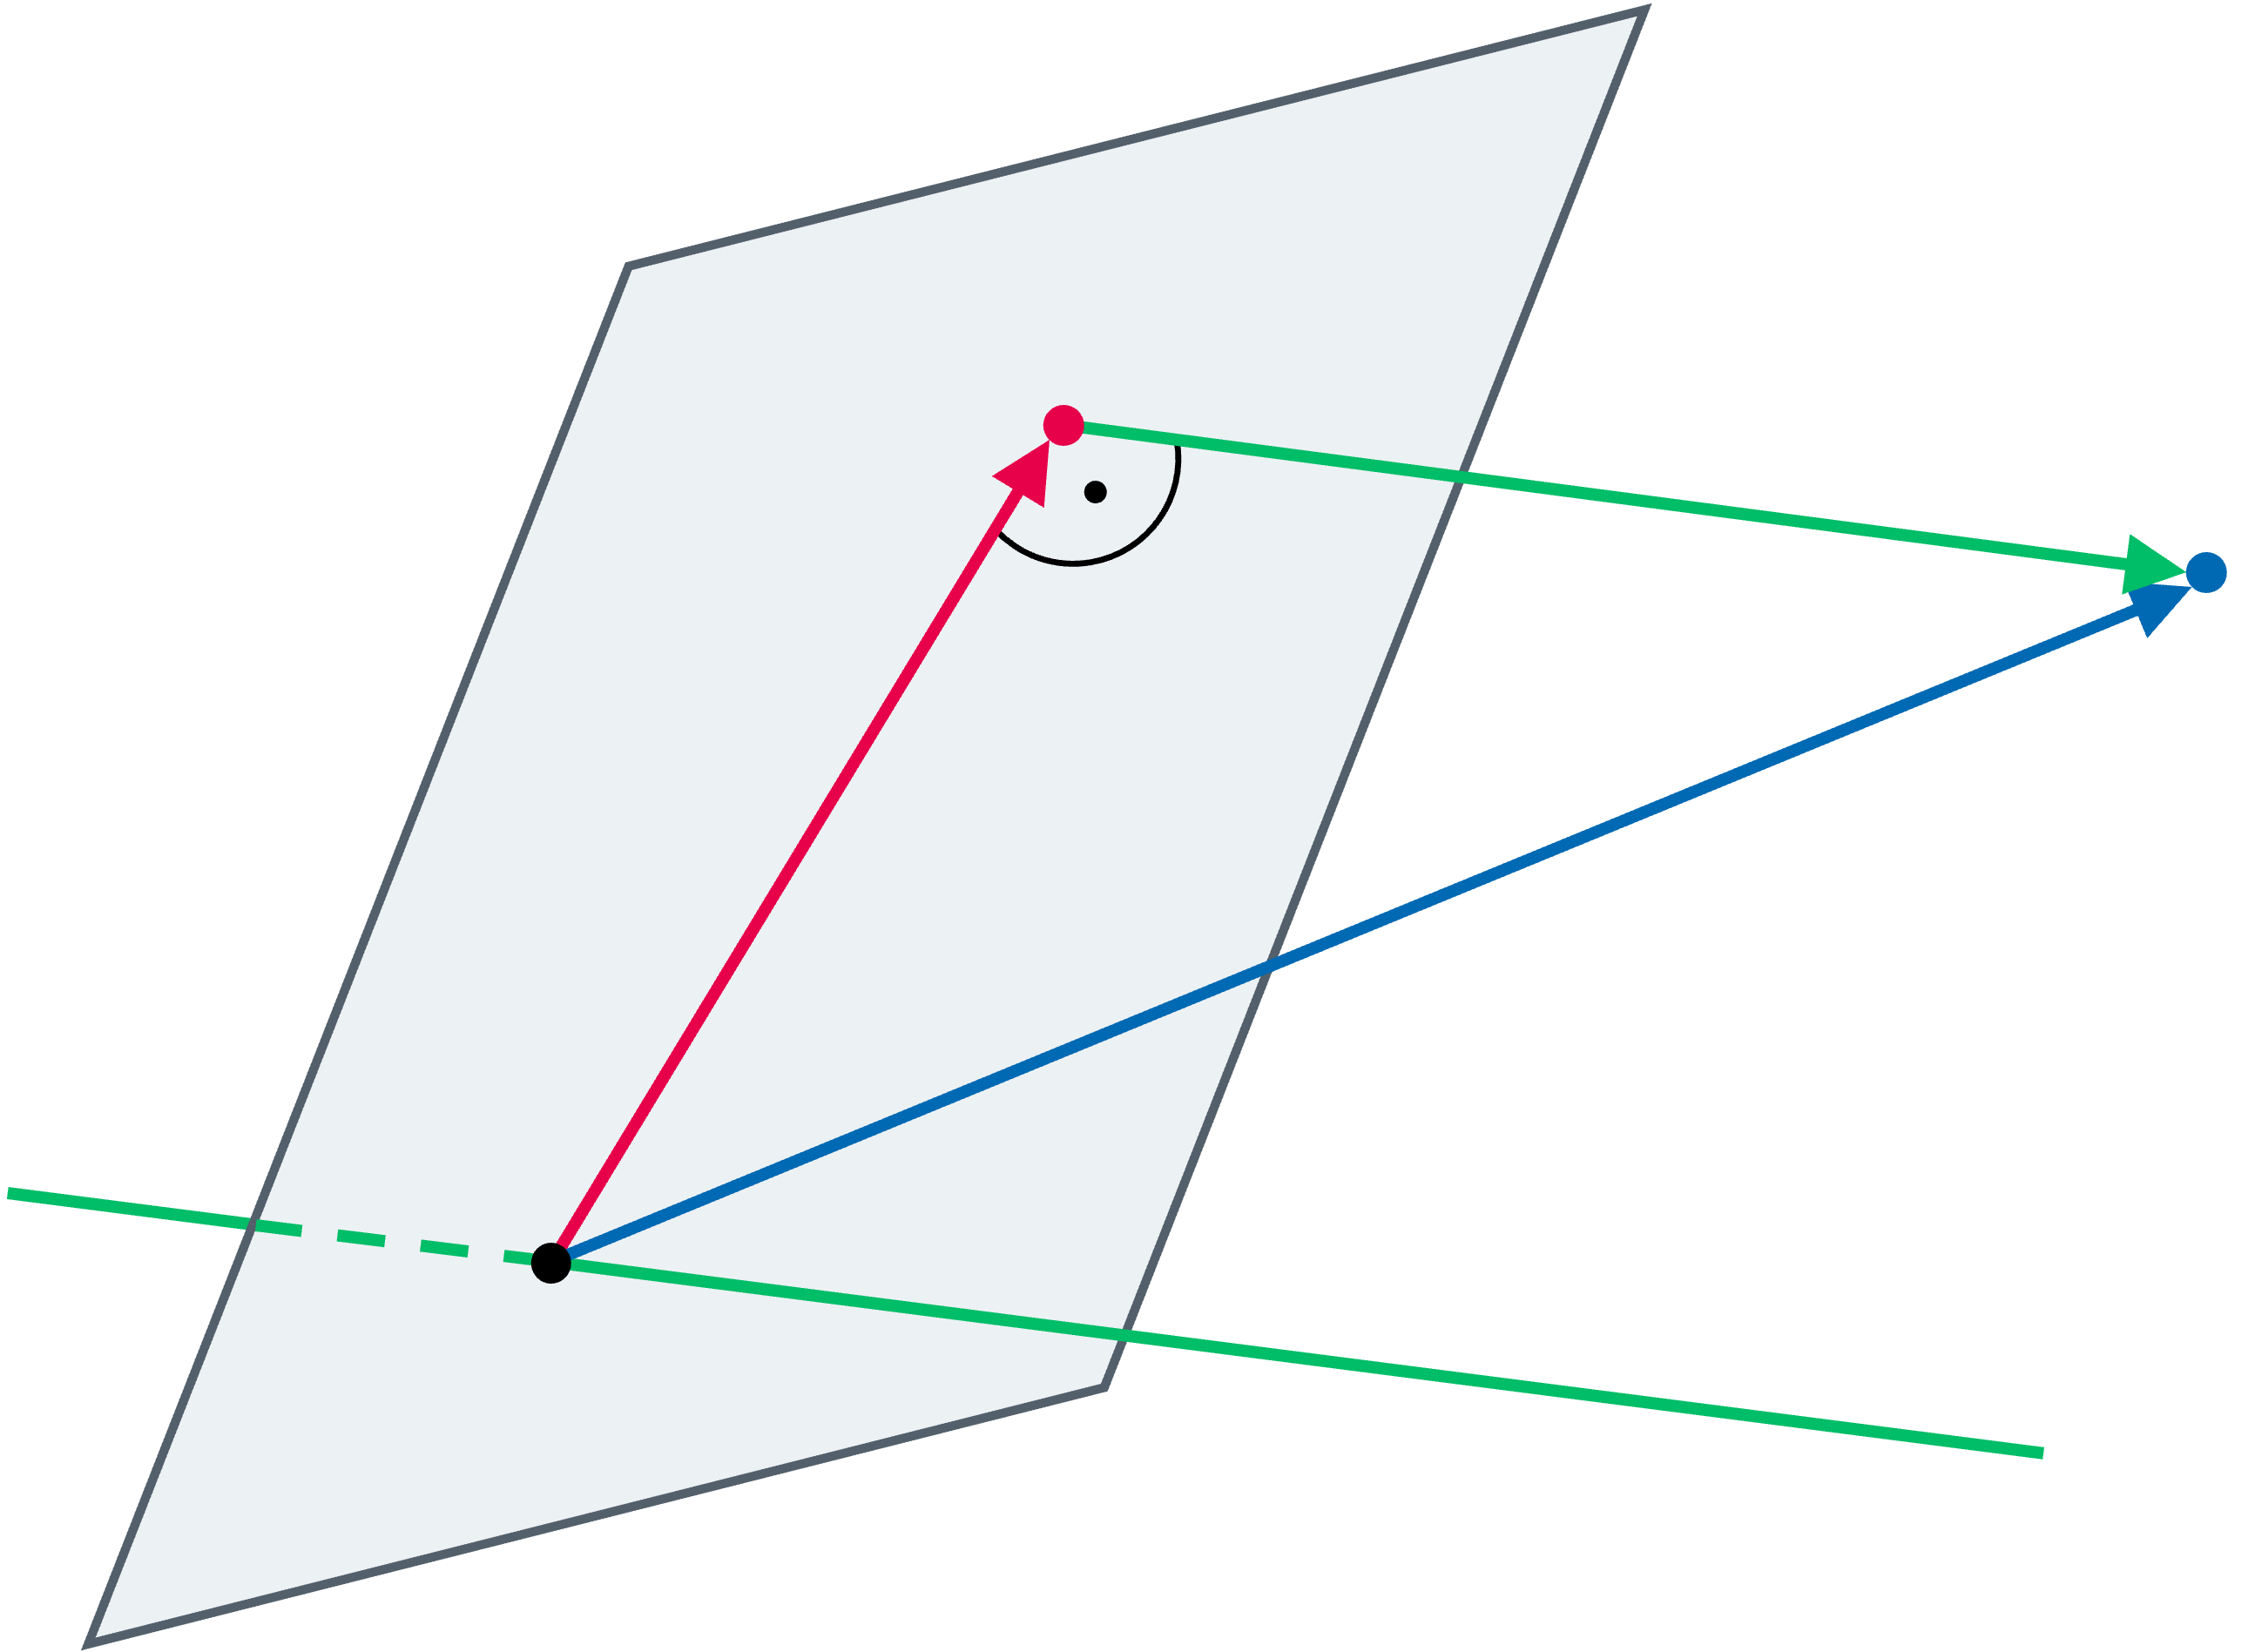
\includegraphics[width=5cm]{other/orthogonal-decomposition}
        };

        % Create scope with normalized axes
        \begin{scope}[
            x={(image.south east)},
            y={(image.north west)}]
         
            % Grid to properly align annotations
            % \draw[help lines, step=0.1] (image.south west) grid ($(image.north east) + (0.001,0)$);

            % Annotate image
            \node[] at (0.22,0.18) {$\mathbf{0}$};
            \node[] at (0.35,0.60) {\color{red} $\mathbf{u}$};
            \node[] at (0.80,0.45) {\color{blue} $\mathbf{v}$};
            \node[] at (0.20,0.75) {\color{red} $U$};
            \node[] at (0.75,0.08) {\color{green} $U^{\bot}$};
            \node[] at (0.80,0.75) {${\color{blue} \mathbf{v}} - {\color{red} \mathbf{u}}$};
        \end{scope}
    \end{tikzpicture}
    \caption{%
         The orthogonal projection ${\color{red} \mathbf{u}} = P({\color{blue} \mathbf{v}})$ of a vector ${\color{blue} \mathbf{v}}$ onto the subspace ${\color{red} U}$. Note that the vector difference ${\color{blue} \mathbf{v}} - {\color{red} \mathbf{u}}$ is orthogonal to the subspace ${\color{red} U}$, i.e., the vector ${\color{red} \mathbf{u}}$ is a vector in ${\color{red} U}$ that minimizes the distance to ${\color{blue} \mathbf{v}}$.
    }
    \label{fig: orthogonal projection}
\end{figure}

Finally, to tie this in with our discussion of conditional expectation, we have to review some (very) fundamental functional analysis as well. For a probability space $(\Omega, \mathcal{A}, \P)$, and $p > 0$, we denote\footnote{Note that $\mathcal{L}^p$ critically depends on the $\sigma$-algebra $\mathcal{A}$ (measurability) and the probability measure $\P$ (integrability), we only drop these in the notation for convenience!} the set of measurable functions $f$ for which $\abs{f}^p$ is integrable with respect to $\P$ by $\mathcal{L}^p$, i.e.,
\[
    \highlightMath{
        \mathcal{L}^p = \set{f \colon \Omega \to \R \with[\Big] f \text{ is measurable, } \int_{\Omega} \abs{f(\omega)}^p \dP(\omega) < \infty}, \quad p > 0.
    }
\]
On $\mathcal{L}^p$, we can define a seminorm via
\[
    \highlightMath{
        \norm{f}_p = \left( \int_{\Omega} \abs{f(\omega)}^p \dP(\omega) \right)^{\nicefrac{1}{p}}, \quad f \in \mathcal{L}^p.
    }
\]
This does \emph{not} yield a \say{true} norm since any two functions $f$ and $g$ that agree almost surely (but may differ on a null set) will share the same seminorm $\norm{f}_p = \norm{g}_p$. In particular, $\norm{f}_p = 0$ does \emph{not} imply $f = 0$ (but only $f = 0$ almost surely). However, this can easily be fixed by considering the set $L^p$ of equivalence classes
\[
    [f] = \set{g \in \mathcal{L}^p \with f \sim g}, \qquad f \sim g \Leftrightarrow \Prob(f - g \neq 0) = 0,
\]
i.e., we simply identify all functions that agree almost surely. On $L^p = \mathcal{L}^p / {\sim}$, we define $\norm{[f]}_p = \norm{f}_p$, and one can check that this indeed defines a norm on $L^p$, turning the latter into a \emph{normed space}. Moreover, one can show (cf. \href{https://en.wikipedia.org/wiki/Riesz–Fischer_theorem#Completeness_of_Lp,_0_%3C_p_≤_∞}{Riesz–Fischer theorem}) that the $L^p$-spaces are \emph{complete} (i.e., every Cauchy sequence converges) with respect to this norm and hence, are \emph{Banach spaces}.

Among all $L^p$-spaces, the space $L^2$ of (equivalence classes of) square-integrable functions is special, as it is the only $L^p$-space that can be equipped with an inner product that induces the norm $\norm{\cdot}_2$ we defined earlier (i.e., $L^2$ is a \emph{Hilbert space}). Indeed, for functions\footnote{For convenience, from now on we will simply speak of functions instead of equivalence classes of functions, and we will also drop the brackets for the equivalence classes.} $f, g \in L^2$, defining
\[
    \highlightMath{
        \langle f, g \rangle_2 = \int_{\Omega} f(\omega) g(\omega) \dP(\omega)
    }
\]
yields an inner product on $L^2$ satisfying $\langle f, f \rangle_2 = \norm{f}_2^2$. Using these newly introduced concepts, the property \eqref{eq: orthogonality of conditional expectation} of the conditional expectation $\Exp[Y \given X]$ can be reformulated as
\[
    \langle Z, Y - \Exp[Y \given X] \rangle_2 = 0,
\]
i.e., the difference between $Y$ and the conditional expectation $\Exp[Y \given X]$ is orthogonal to every $\sigma(X)$-measurable, integrable random variable $Z$. Moreover, note that the space of $\sigma(X)$-measurable, square-integrable random variables is a subspace of all square-integrable random variables on $(\Omega, \mathcal{A}, \P)$. Since the conditional expectation $\Exp[Y \given X]$ is, by definition, also $\sigma(X)$-measurable, identity \eqref{eq: orthogonality of conditional expectation} thus implies that the conditional expectation of $Y$ given $X$ is the orthogonal projection of $Y$ onto the subspace of $\sigma(X)$-measurable, square-integrable random variables on $(\Omega, \mathcal{A}, \P)$. As discussed earlier, this also implies that $\Exp[Y \given X]$ is the random variable in the space of $\sigma(X)$-measurable, square-integrable random variables that is closest to $Y$ with respect to the norm $\norm{\cdot}_2$. In other words, taking into account all the information provided by the input $X$, the conditional expectation $\Exp[Y \given X]$ is our best guess at the value of the output $Y$.

Finally, note that the conditional expectation $\Exp[Y \given X]$ depends on $X$ only via the $\sigma$-algebra $\sigma(X)$ generated by $X$, and, indeed, it makes perfect sense to define the conditional expectation of $Y$ given a sub-$\sigma$-algebra $\mathcal{F} \subset \mathcal{A}$. Also, one can prove existence of the conditional expectation $\Exp[Y \given \mathcal{F}]$ assuming that $\Exp[\abs{Y}] < \infty$.

To conclude this intermezzo on conditional expectation, we list some\footnote{Note that this is merely a selection. In fact, there are many other useful properties of conditional expectation, such as monotone convergence, dominated convergence, Fatou's lemma, Jensen's inequality, and many more.} important properties\footnote{Again, these identities/inequalities are to be understood in an almost sure sense.} of conditional expectation:

\begin{itemize}
    \label{itm: properties of conditional expectation}
    \item $\Exp[\Exp[Y \given \mathcal{F}]] = \Exp[Y] \quad$ (law of total expectation)

    \item $\Exp[\lambda Y + Z \given \mathcal{F}] = \lambda \Exp[Y \given \mathcal{F}] + \Exp[Z \given \mathcal{F}] \quad$ (linearity)

    \item If $Y \leq Z$, then $\Exp[Y \given \mathcal{F}] \leq \Exp[Z \given \mathcal{F}] \quad$ (monotonicity)

    \item If $Y$ is independent of $\sigma(Z, \mathcal{F})$, then $\Exp[YZ \given \mathcal{F}] = \Exp[Y] \Exp[Z \given \mathcal{F}] \quad$ (pulling out independent factors)
    
    \item In particular, if $Y$ is independent of $\mathcal{F}$, then $\Exp[Y \given \mathcal{F}] = \Exp[Y] \quad$ (pulling out independent factors)

    \item If $Y$ is $\mathcal{F}$-measurable, then $\Exp[Y \given \mathcal{F}] = Y \quad$ (stability)

    \item In particular, for sub-$\sigma$-algebras $\mathcal{F}_1 \subset \mathcal{F}_2 \subset \mathcal{A}$, we have $\Exp[\Exp[Y \given \mathcal{F}_1] \given \mathcal{F}_2] = \Exp[Y \given \mathcal{F}_1] \quad$ (stability)

    \item If $Y$ is $\mathcal{F}$-measurable, then $\Exp[YZ \given \mathcal{F}] = Y \Exp[Z \given \mathcal{F}] \quad$ (pulling out known factors)

    \item For sub-$\sigma$-algebras $\mathcal{F}_1 \subset \mathcal{F}_2 \subset \mathcal{A}$, we have $\Exp[\Exp[Y \given \mathcal{F}_2] \given \mathcal{F}_1] = \Exp[Y \given \mathcal{F}_1] \quad$ (tower rule)
\end{itemize}

In the previous section, we claimed that mean squared error and conditional expectation are closely related to each other. The following result makes this relationship explicit. Before we state the result, note that the conditional expectation of $Y \in \R^d$ given $X$ is simply the vector of conditional expectations of $Y_i$ given $X$ for $i = 1, \dots, d$, i.e.,
\[
    \Exp[Y \given X] = (\Exp[Y_1 \given X], \dots, \Exp[Y_d \given X])^{\top}.
\]
We have the following result:

\begin{proposition}
\label{prop: decomposition of mean-squared error}
Let $Y \colon \Omega \to \R^d$ be a random variable such that $\Exp[\abs{Y_i}] < \infty$, $i = 1, \dots, d$, and let $X \colon \Omega \to \mathcal{X}$ be a random variable and $f \colon \mathcal{X} \to \R^d$ a measurable function such that the mean squared error $\MSE(f)$ exists. Then,
\[
    \MSE(f) = \MSE(f, \Exp[Y \given X]) + \Exp[\sigma_Y^2(X)],
\]
where
\[
    \sigma_Y^2(X) = \Exp[\norm{Y - \Exp[Y \given X]}_2^2 \given X]
\]
is the \emph{conditional variance} of $Y$ given $X$. In particular,
\[
    \MSE(\Exp[Y \given X]) = \Exp[\sigma_Y^2(X)] = \Exp[\norm{Y - \Exp[Y \given X]}_2^2].
\]
\end{proposition}

\begin{proof}
Bilinearity of the inner product yields
\begin{align*}
    \MSE(f) &= \Exp[\norm{f(X) - Y}_2^2] = \Exp[\norm{(f(X) - \Exp[Y \given X]) + (\Exp[Y \given X] - Y)}_2^2] \\
    &= \Exp[\norm{f(X) - \Exp[Y \given X]}_2^2] + \Exp[\norm{\Exp[Y \given X] - Y}_2^2] + 2 \sum_{i=1}^d \Exp[(f_i(X) - \Exp[Y_i \given X]) (\Exp[Y_i \given X] - Y_i)].
\end{align*}
The terms $\Exp[(f_i(X) - \Exp[Y_i \given X]) (\Exp[Y_i \given X] - Y_i)]$ vanish for $i = 1, \dots, d$. By the law of total expectation, we have
\[
    \Exp[\norm{\Exp[Y \given X] - Y}_2^2] = \Exp[\norm{Y - \Exp[Y \given X]}_2^2] = \Exp[\Exp[\norm{Y - \Exp[Y \given X]}_2^2 \given X]] = \Exp[\sigma_Y^2(X)].
\]
Altogether,
\[
    \MSE(f) = \Exp[\norm{f(X) - \Exp[Y \given X]}_2^2] + \Exp[\norm{\Exp[Y \given X] - Y}_2^2] = \MSE(f, \Exp[Y \given X]) + \Exp[\sigma_Y^2(X)]. \qedhere
\]
\end{proof}

\begin{remark}
\label{rmk: input-output}
\begin{enumerate}
    \item The quantity $\MSE(f, \Exp[Y \given X])$ measures the mean squared error of using $f(X)$ as an approximation of the conditional expectation $\Exp[Y \given X]$.

    \item The term $\Exp[\sigma_Y^2(X)]$ is independent of the choice of $f \colon \mathcal{X} \to \R^d$. In particular, this shows that the mean squared error $\MSE(f)$ is minimized by $f(X) = \Exp[Y \given X]$.

    \item The property $\P_{(X, Y)} = \P_{Y \given X} \P_X$ enables us to consider $\mathcal{X} \times \mathcal{Y}$ sequentially, i.e., as an input space $\mathcal{X}$ \emph{followed} by an output space $\mathcal{Y}$, since, for any measurable function $f \colon \mathcal{X} \times \mathcal{Y} \to \R$, we have
        \[
            \Exp[f(X, Y)] = \int_{\mathcal{X}} \left( \int_{\mathcal{Y}} f(x, y) \dP_{Y \given X=x}(y) \right) \dP_X(x).
        \]
\end{enumerate}
\end{remark}
